\documentclass[11pt, a4paper]{article}
\usepackage{amsfonts, amsmath, hanging, hyperref, natbib, parskip, times}
\usepackage[pdftex]{graphicx}
\hypersetup{
  colorlinks,
  linkcolor=blue,
  urlcolor=blue
}

\usepackage{wrapfig}

\let\section=\subsubsection
\newcommand{\pkg}[1]{{\normalfont\fontseries{b}\selectfont #1}} 
\let\proglang=\textit
\let\code=\texttt 
\renewcommand{\title}[1]{\begin{center}{\bf \LARGE #1}\end{center}}
\newcommand{\affiliations}{\footnotesize}
\newcommand{\keywords}{\paragraph{Keywords:}}

\setlength{\topmargin}{-15mm}
\setlength{\oddsidemargin}{-2mm}
\setlength{\textwidth}{165mm}
\setlength{\textheight}{250mm}

\begin{document}
\pagestyle{empty}

\title{\pkg{likert}: An R Package for Visualizing and Analyzing Likert-Based Items}

\begin{center}
  {\bf Kimberly K. Speerschneider$^{1,2,^\star}$}\\
  {\bf Jason M. Bryer$^{1,2}$}
\end{center}

\begin{affiliations}
1. University at Albany \\[-2pt]
2. Excelsior College \\[-2pt]
$^\star$Contact author: \href{mailto:kimkspeer@gmail.com}{kimkspeer@gmail.com}
\end{affiliations}

\keywords likert, questionnaire data, visualization, grammar of graphics

\vskip 0.8cm

The Likert \citep{Likert1932} item format has become the \textit{defacto} standard in survey research. In the most common format of Likert-items, respondents rate their agreement with a statement from strongly disagree to strongly agree, usually with four to seven levels. Rensis Likert assumed that the distance between each response category are equal, and as such, analysis has typically treated the responses to Likert-items as continuous variables. However, this assumption often does not hold \citep[see e.g.][]{Wakita2012}, although can often easily be verified with the use of visualizations. This talk introduces the \pkg{likert} package that provides a set of functions for analyzing Likert-items, visualizing results using the \pkg{ggplot2} \citep{ggplot2} package, and reporting results with the \pkg{xtable} \citep{xtable} package. Figure 1 represents one such graphic analyzing reading attitudes from the Programme of International Student Assessment \citep[PISA;][]{pisa}

\begin{figure}[h!]
\begin{center}
    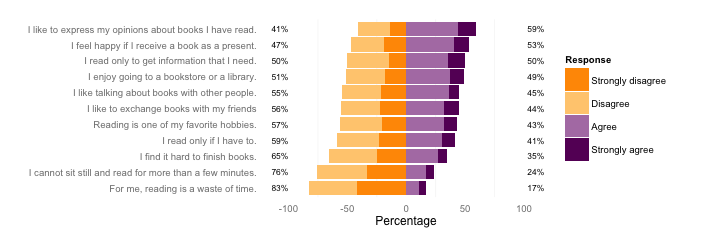
\includegraphics[width=\textwidth]{likert-l28}
    \caption{Attitudes Towards Reading}
    \end{center}
    \label{likertplot}
\end{figure}

%% references: 
%\nocite{ImaivanDyk2004,Zhaoetal2012}
\bibliographystyle{chicago}
\bibliography{likert}

\end{document}
